\newpage
\section{Reduction}


\begin{figure}[H]
    \centering
    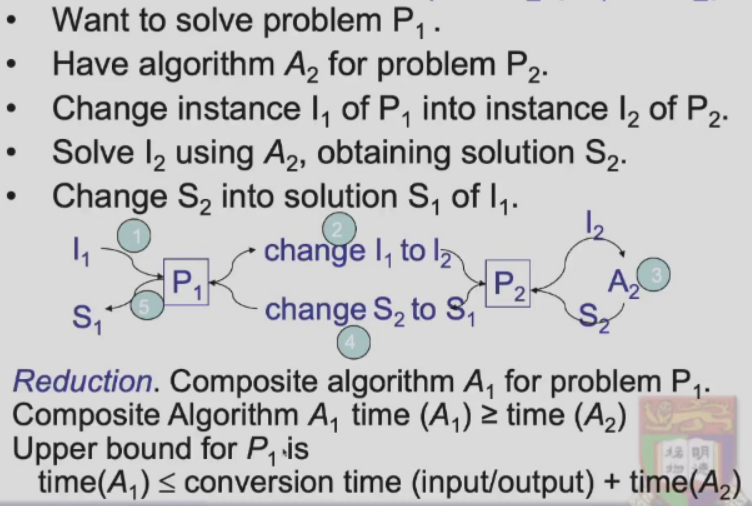
\includegraphics[width=0.309\textwidth]{pic/DAA6/Problem reduction}
    \caption{Problem reduction $P_1$ to $P_2$.($P_1\propto P_2$)}
\end{figure}

\subsection{Lower Bound by Reduction}
\begin{figure}[H]
    \centering
    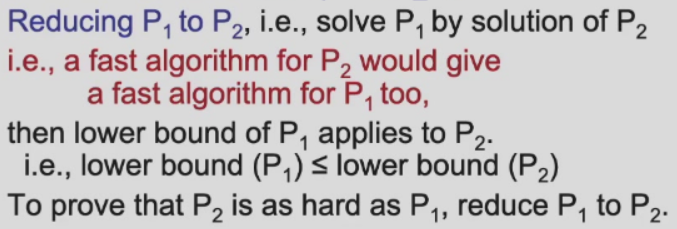
\includegraphics[width=0.309\textwidth]{pic/DAA6/Lower Bound by Reduction}
    \caption{Lower Bound by Reduction}
\end{figure}


\subsection{Distinct Integers Sorting}
\begin{figure}[H]
    \centering
    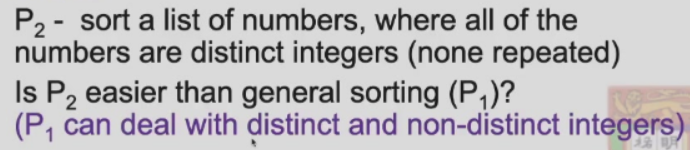
\includegraphics[width=0.309\textwidth]{pic/DAA6/Distinct Integers Sorting1}
    \caption{Distinct Integers Sorting}
\end{figure}

\begin{theorem}
    Distinct integer sorting is not easier
\end{theorem}

\begin{figure}[H]
    \centering
    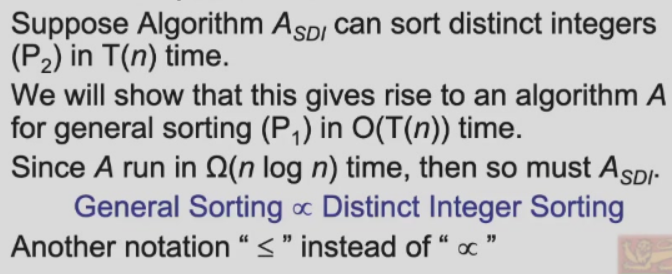
\includegraphics[width=0.309\textwidth]{pic/DAA6/proof}
    \caption{proof}
\end{figure}

\begin{figure}[H]
    \centering
    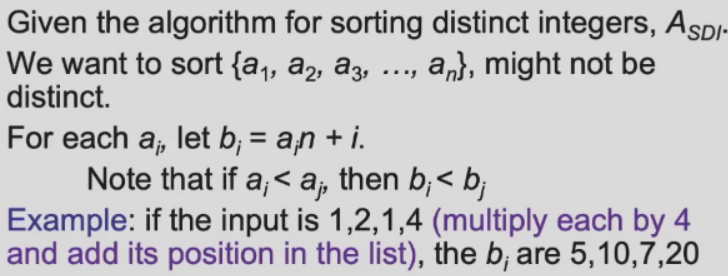
\includegraphics[width=0.309\textwidth]{pic/DAA6/How to build A from ASDI}
    \caption{How to build $A$ from $A_{SDI}$}
\end{figure}


\begin{figure}[H]
    \centering
    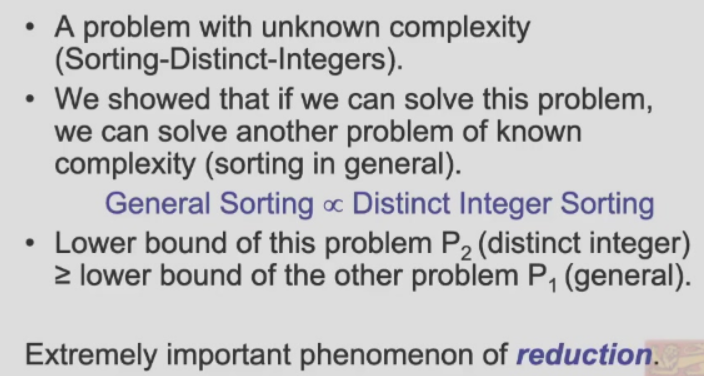
\includegraphics[width=0.309\textwidth]{pic/DAA6/phenomenon reduction}
    \caption{phenomenon reduction}
\end{figure}


\subsection{Proof of NP-completeness}

\begin{figure}[H]
    \centering
    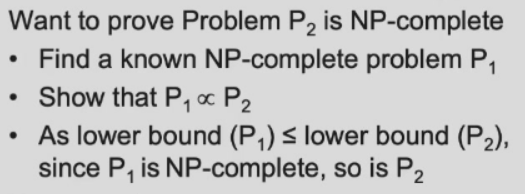
\includegraphics[width=0.309\textwidth]{pic/DAA6/Proof of NP-completeness}
    \caption{Proof of NP-completeness}
\end{figure}

\begin{figure}[H]
    \centering
    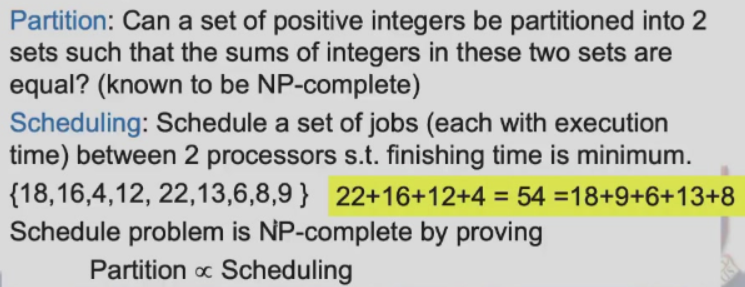
\includegraphics[width=0.309\textwidth]{pic/DAA6/example np}
    \caption{Example}
\end{figure}



\subsection{Integer Distinctness Problem}
\begin{figure}[H]
    \centering
    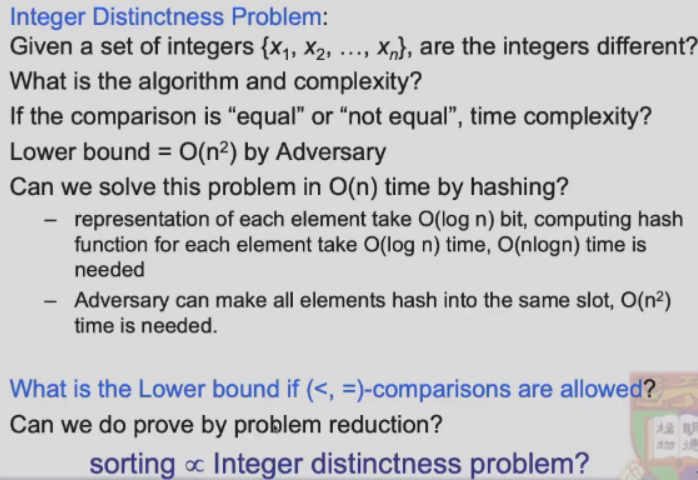
\includegraphics[width=0.309\textwidth]{pic/DAA6/Integer Distinctness Problem}
    \caption{Integer Distinctness Problem}
\end{figure}

计算 hash 也有复杂度, 一般是个大于 $\log n$ 的常数.

\begin{figure}[H]
    \centering
    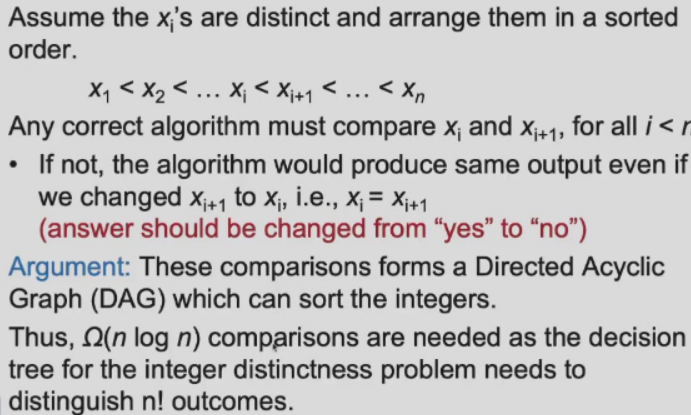
\includegraphics[width=0.309\textwidth]{pic/DAA6//Integer Distinctness Problem1}
    \caption{Integer Distinctness Problem}
\end{figure}


\subsubsection{Closest Pair Problem}

\begin{figure}[H]
    \centering
    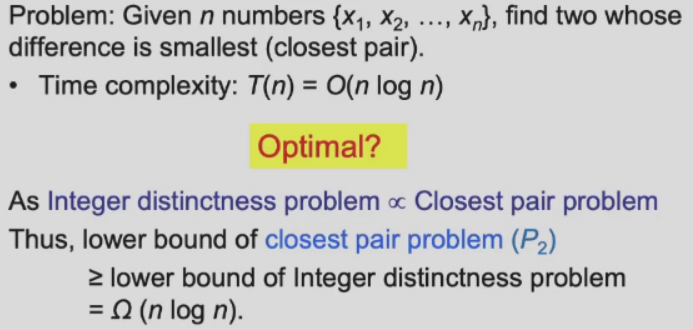
\includegraphics[width=0.309\textwidth]{pic/DAA6/Closest Pair Problem}
    \caption{Closest Pair Problem}
\end{figure}

\subsection{Data Compression}

\begin{figure}[H]
    \centering
    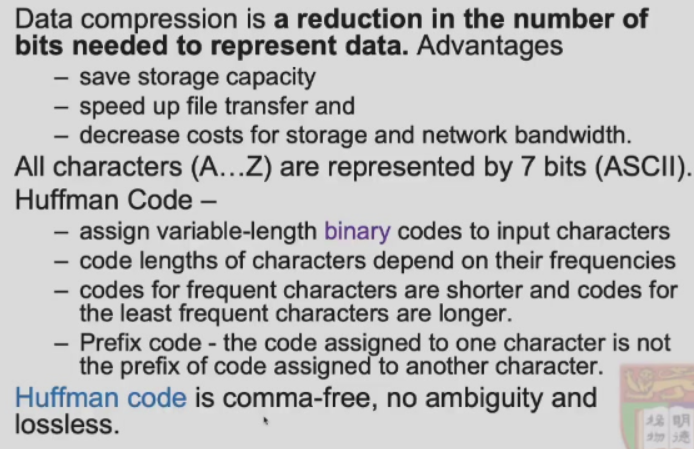
\includegraphics[width=0.309\textwidth]{pic/DAA6/Data Compression}
    \caption{Data Compression}
\end{figure}

\subsubsection{Huffman code}
\begin{figure}[H]
    \centering
    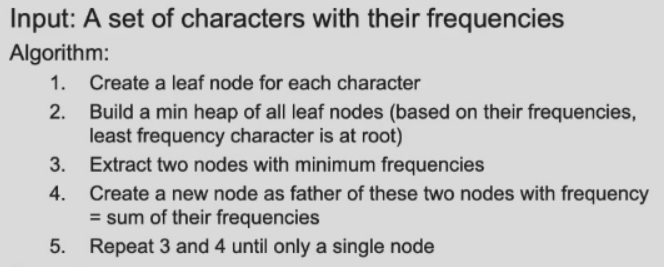
\includegraphics[width=0.309\textwidth]{pic/DAA6/Huffman code}
    \caption{Huffman code}
\end{figure}
Complexity: $O(n\log n)$

%TODO 5.11 没回放, 没法截屏 ppt 了, 就只打个标题, 后面补充了.

\subsubsection{Lower Bound for Huffman}
convert $x_i$ with $y_i=2^{x_i}$


\subsection{3SUM Problem}
$a+b+c=0$?

example and sketch proof

目前最佳的算法, 但下界没有被证明

\subsubsection{Collinearity}
3SUM $\propto$ General Collinearity




Another proof 



\subsubsection{Segment Splitting Problem}
3SUM $\propto$ Collinearity $\propto$ Segment Splitting

gadgets 


\subsubsection{Motion Planning}
3SUM $\propto$ Collinearity $\propto$ Segment Splitting $\propto$ Motion Planning



% 5.14 的
\subsubsection{M-3SUM and 3SUM are Equivalent}
